\chapter{Hardware design}
The hardware chapter describes the different physical objects that have been designed and realized. 
\section{Power line and switch mode}
\writer{Dennis Madsen}
%
The full documentation for the \textit{power line and switch mode} circuit board can be found in appendix\footnote{EPRO\_3\_\&\_4\_PLC - Hardware.pdf}. The board has been designed to have good EMC qualities, which is documented in a report for it self\footnote{EEMC1 report}.
\p Figure \ref{fig:plc_and_smps} shows the division of the circuit board.
\\ Connections:
\begin{itemize}
	\item 30VDC: Connection to the 30V (+/- 10 \%) power line. Used to create a 5 volt supply to power up the micro controller - and the FPGA board.
	\item 5VDC: the two plugs are connected in parallel. However only 3 Amperes must be drawn from each connector due to the track widths.
	\begin{itemize}
		\item If both switch mode power supplies are mounted on the PCB, the total output current is maximum 6 Amperes.
	\end{itemize}
	\item Config Jumpers - jumper 1: Switch between normal mode and write to register mode.
	\item Config Jumpers - jumper 2: Switch between two different communication frequencies.
	\item ARM signals: Power Line control signals (Sleep, Wake up, reset), communication (uart tx and rx) and 3v3 supply to the power line device.
\end{itemize}

\begin{figure}[H]
	\begin{centering}
		 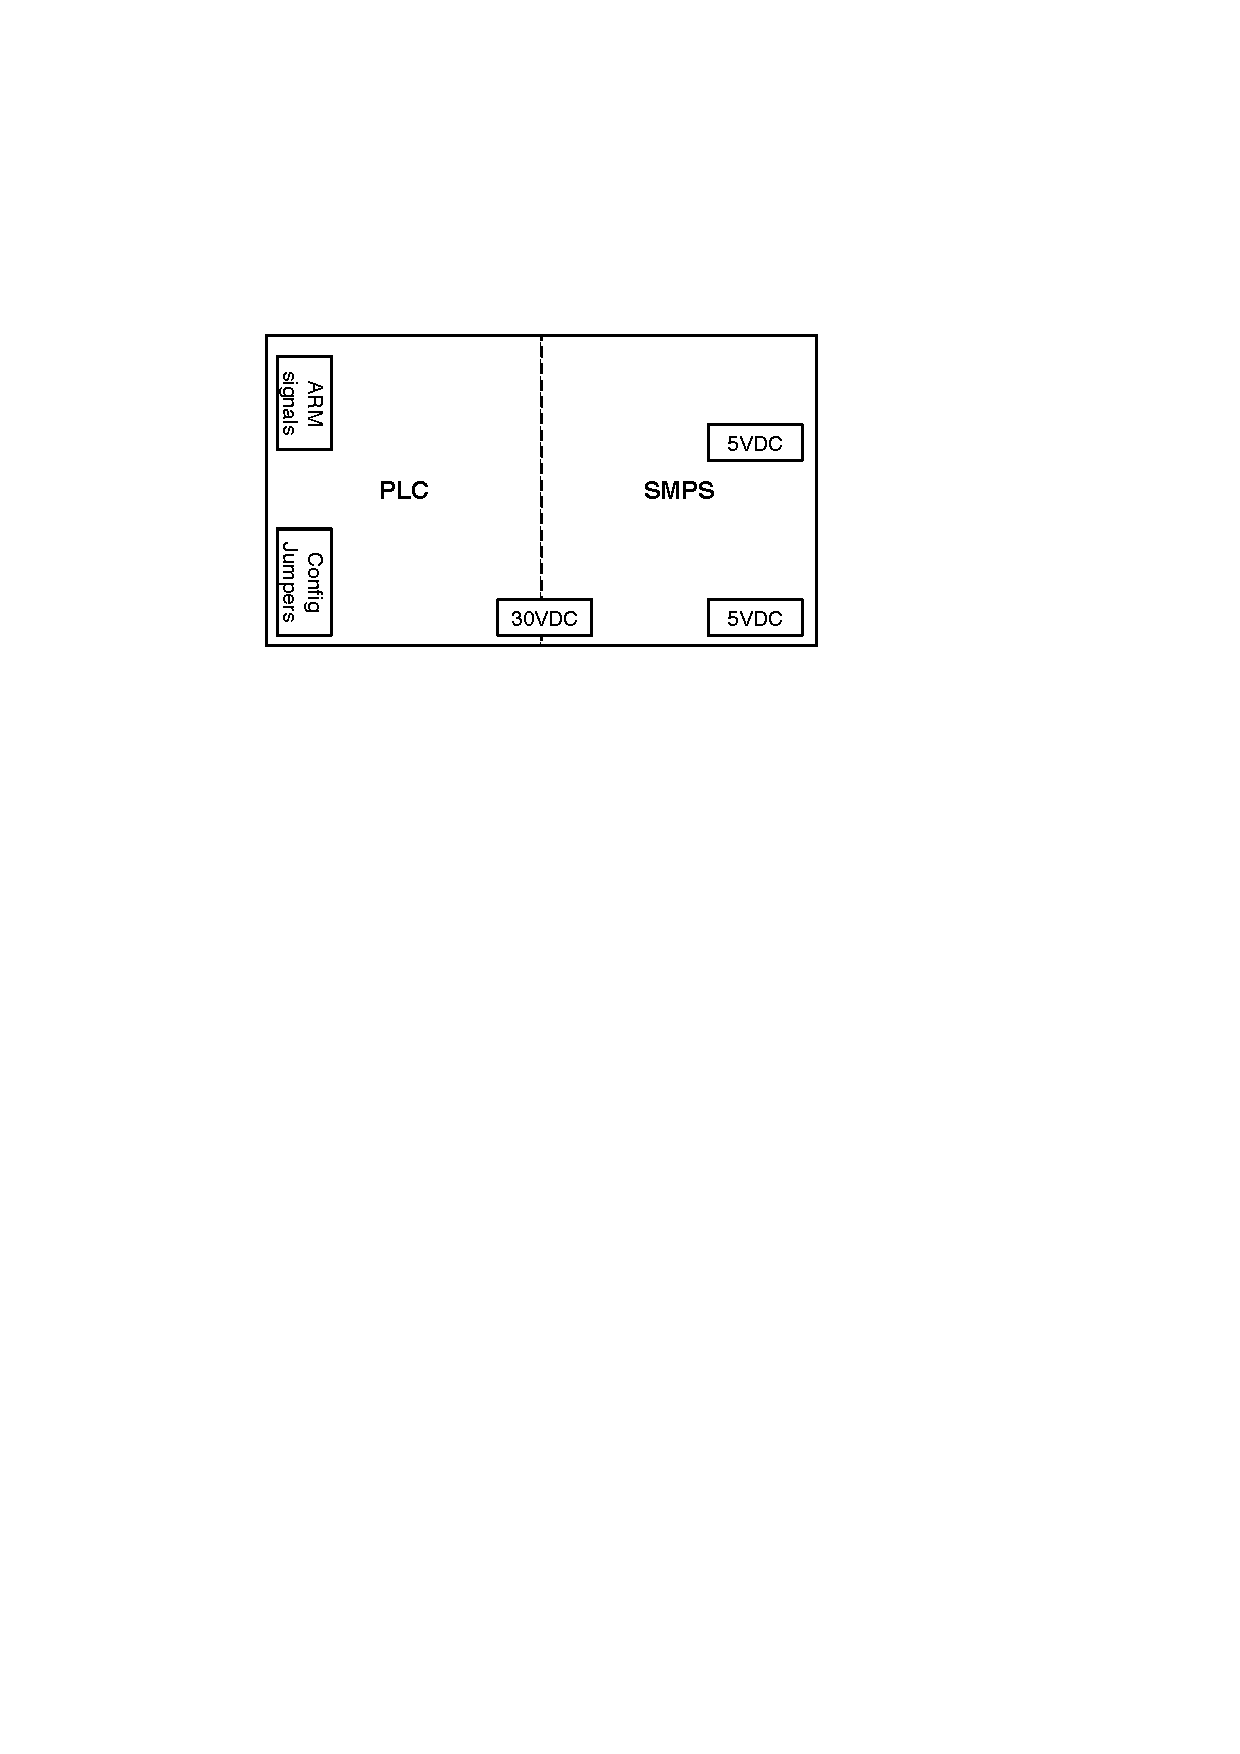
\includegraphics[width=0.60\textwidth]{images/hw_plc_pcb_layout.pdf}
		\caption{Division of the Power line and switch mode device.}
		\label{fig:plc_and_smps}
	\end{centering}
\end{figure}
Figure \ref{fig:plc_and_smps_pic} shows the mounted board with both switch mode supplies mounted and explanation text for all pins.
\begin{figure}[H]
	\begin{centering}
		 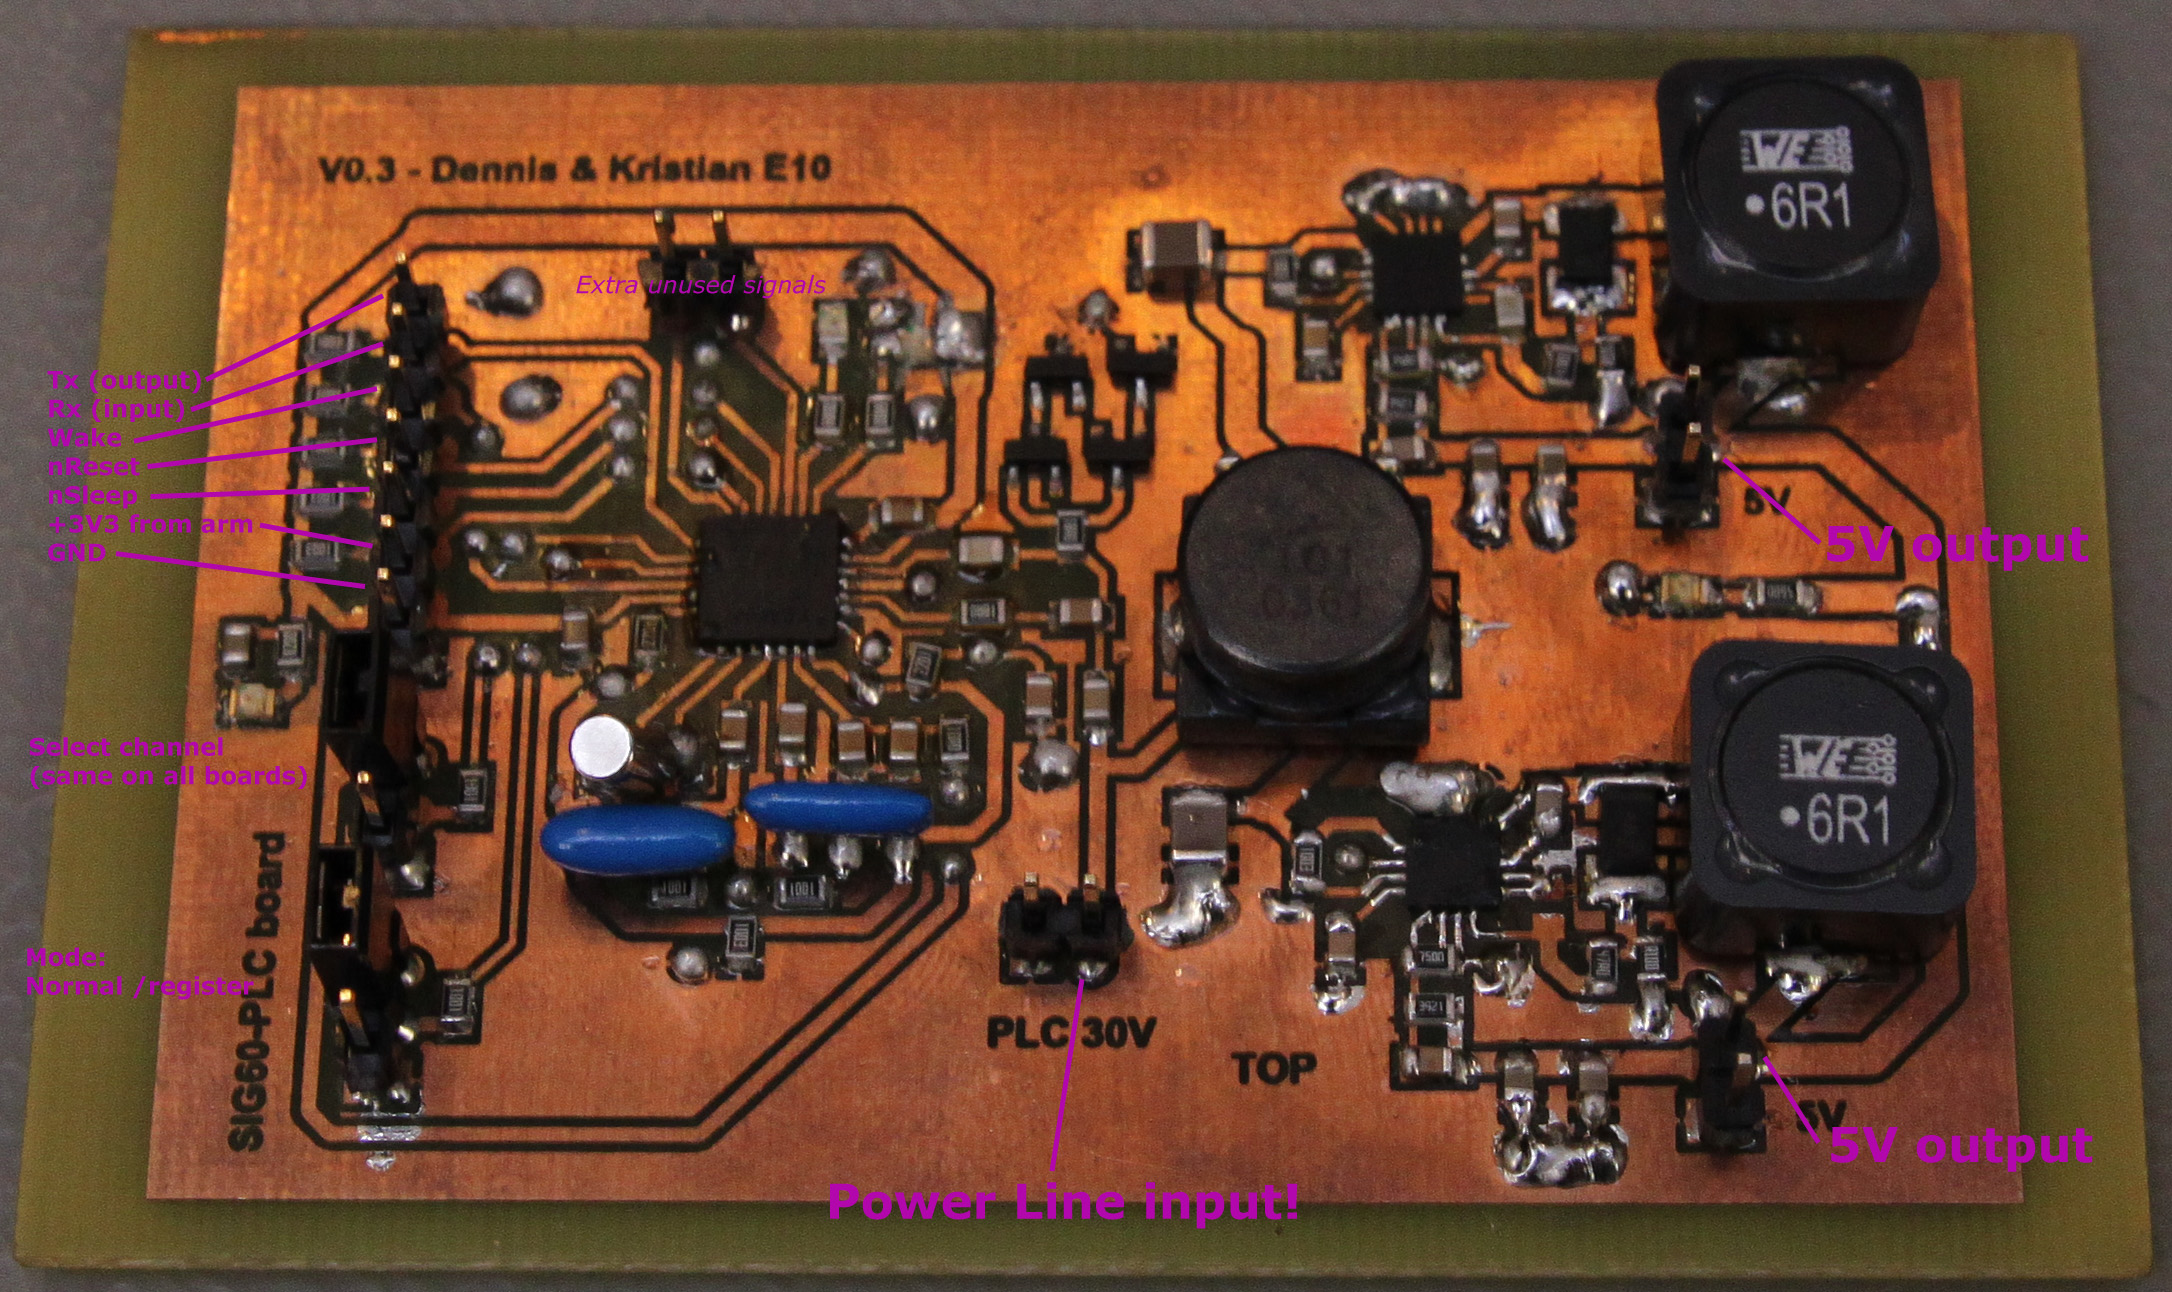
\includegraphics[width=0.90\textwidth]{images/hw_plc_image.jpg}
		\caption{Power Line Communication and DC/DC switch mode PCB.}
		\label{fig:plc_and_smps_pic}
	\end{centering}
\end{figure}



\section{Power switch}
\writer{Paulo Fontes}
%

\section{Interface}
\writer{Dennis Madsen}
According to chapter \ref{chap:digital_design} section \ref{sec:arm_to_fpga}, an interface board has been designed to connect the ARM processor with the FPGA. 
The design is described in \textit{time box 1}. Figure \ref{fig:arm2fpga_interface} shows the final mounted PCB
\p Beside interfacing the processor to the FPGA, the board also interfaces to the power line module. 
\p All unused pins from the pin headers J1 and J2 are routed to another pin header where some of the pins are used to control the power switches connected.
 
\begin{figure}[H]
	\begin{centering}
		 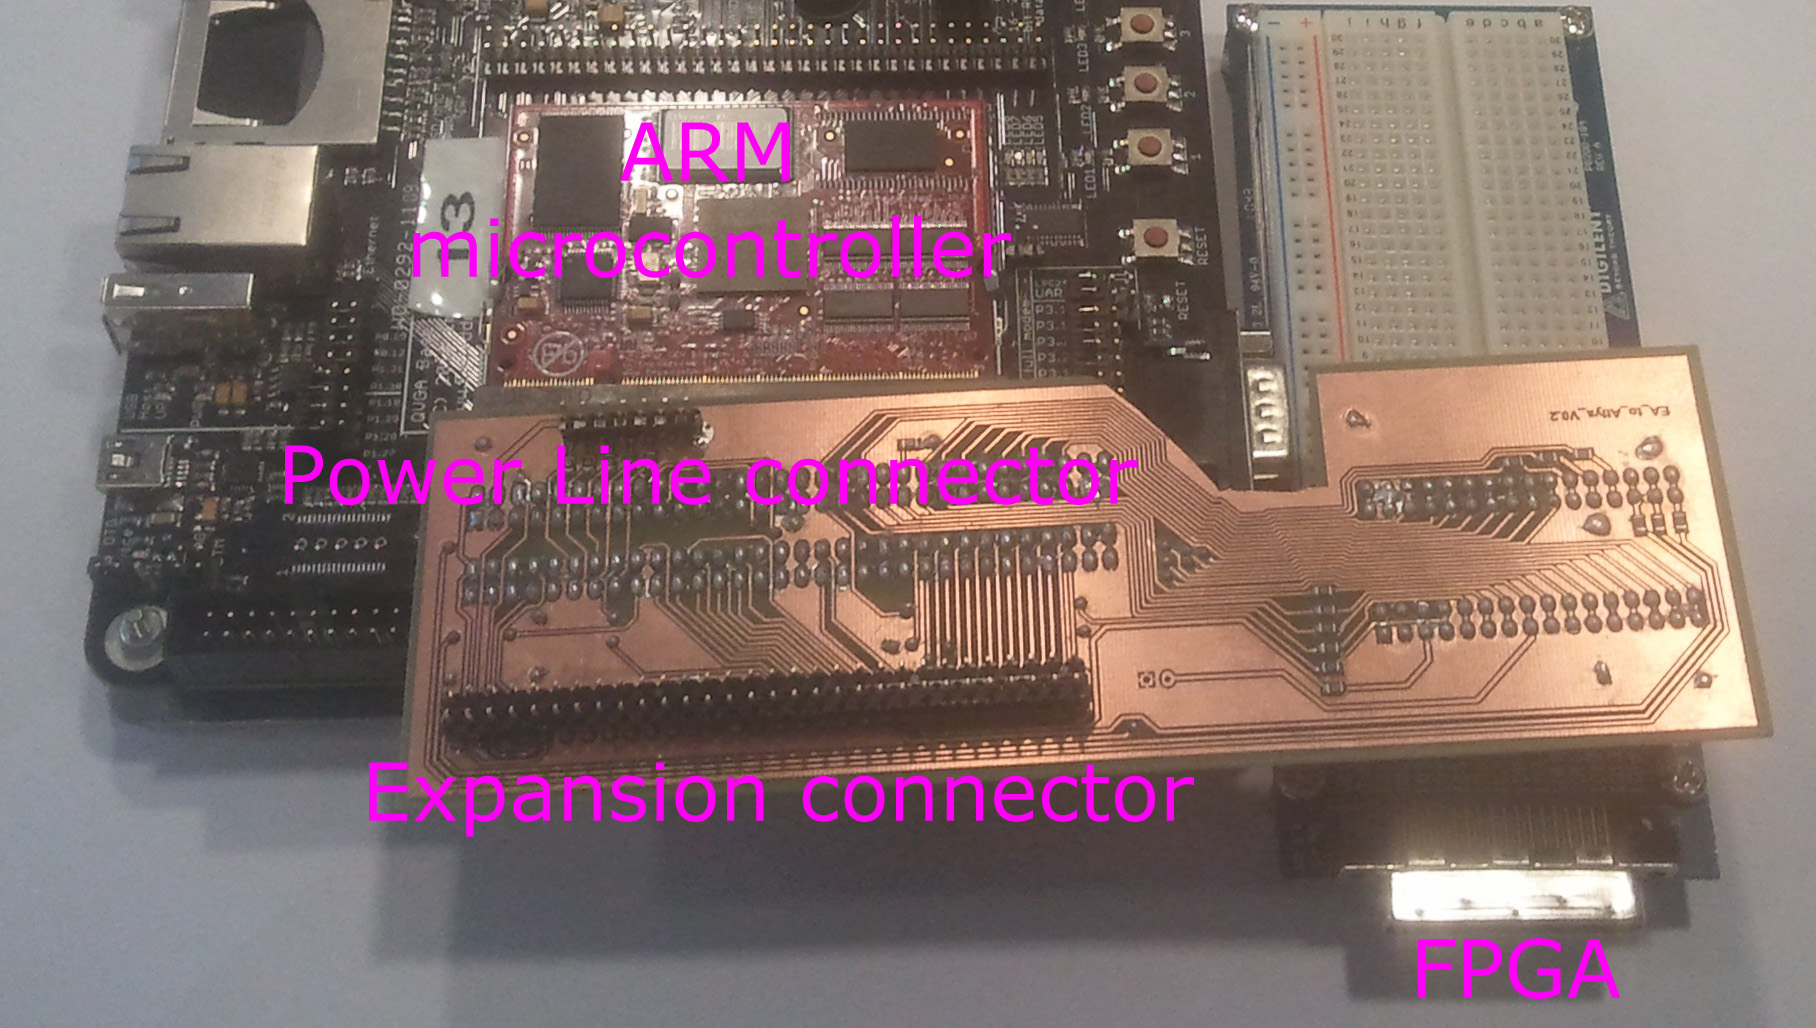
\includegraphics[width=0.80\textwidth]{images/hw_interface_photo_v0_2.jpg}
		\caption{Picture of the ARM to Spartan6 interface PCB.}
		\label{fig:arm2fpga_interface}
	\end{centering}
\end{figure}
